\section{Assumptions}\label{sec:assumptions}
\subsection{Top Down}\label{subsec:assumptions_top_down}
\subsection{Bottom Up}\label{subsec:assumptions_bottom_up}
\subsection{Value Theory}\label{subsec:assumptions_value_theory}
To illustrate how the python code exports the figures directly into the report, this second "hw2" is included. Below are the pictures that are created by the code listed in \cref{app:1} and \cref{app:2}.
\begin{figure}[H]
    \centering
    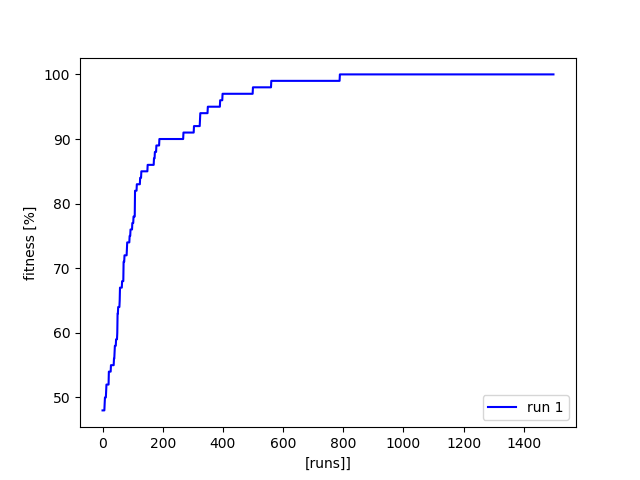
\includegraphics[width=1\textwidth]{Images/4a.png}
    \caption{Performance of some genetic algorithm}
\end{figure}

\begin{figure}[H]
    \centering
    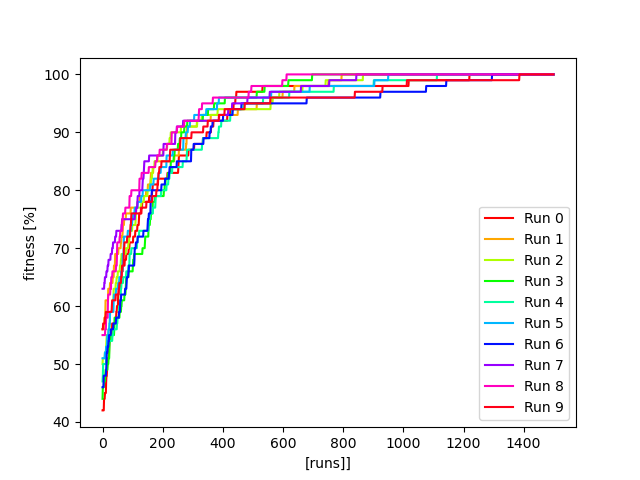
\includegraphics[width=1\textwidth]{Images/4b.png}
    \caption{Performance of some genetic algorithm}
\end{figure}